In recent years, there has been a substantial increase in interest of open source projects. Open source software is typically developed by community of people interested in the particular area who don't necessarily know each other. These communities are usually web-based.The open-source phenomenon raises many interesting questions. Its pro-ponents regard it as a paradigmatic change whereby the economics of private goods, built on the scarcity of resources, is replaced by the economics of public goods, where scarcity is not an issue. \cite{alexander2002working} There are many other projects which are on top of their game and yet still being open source. For example, Apache, a free server program is often a go-to decision when for a web server implementation and in 2002 it was used on 56\% of web servers worldwide \cite{lerner2001open}.

\section{History of Open-Source Software}
When talking about open source, most people immediately think of Linux. But there's so much more than than. The origin of open-source software can be traced back to the 1950s and 1960s, when software was sold together with hardware, and macros and utilities were freely exchanged in user forums. \cite{alexander2002working} In late 1983, GNU project has been announced and the next year a Free Software Foundation has been founded - both by an MIT employee Richard M. Stallman. All software written and released under Free Software Foundation had zero licences. The Linux kernel was released as freely modifiable source code in 1991 and like Unix, it attracted attention from many volunteer programmers. Another big milestone was a year 1998 when Netscape released a source code for Mozilla. In 1999 it was obvious that more and more corporate money will be invested into open source space as IBM announced their support for Linux by investing \$1 billion in its development.

\section{Choosing projects of interest}
There are loads of OSS projects nowadays and it turned out to be pretty interesting process to choose the correct ones for my project. To make sure chosen projects fit into my work and fit  all my needs I defined several requirements which needed to be fulfilled at least to some extent:

\begin{itemize}
  \item Project needs to be widely used and well-known. This ensures there will be enough data on social media about it what will result in the less biased final results.
  \item Project has to have accessible bug tracking system or Git repository with list of known issues. This will provide the data for pairing the social media data with their corresponding bug items.
  \item Ideally, projects could be from the same area to avoid coincidentally choosing an outlier project from some either popular or unpopular field.
\end{itemize}

After considering these three points, I ended up choosing several open source web development frameworks as my projects of interest. 

Project of my choice are NodeJS, AngularJS, EmberJS, VueJS for frontend technologies and Laravel, Symfony and CakePhp for backend PHP technologies. Some frameworks like Django, Meteor, React have been left out because of their misleading names  would require lot of additional work to filter out data unrelated to the actual frameworks. For example, when tested Django framework, most of the twitter data referred to movie "Django Unchained".

Other very interesting group of OSS project to examine are cryptocurrencies. Being a very hot topic these days, I've decided to work with some of the most popular cryptocurrency repositories as well. These were Bitcoin, Ethereum, Litecoin, Dash and Ripple.

\section{Github mining}
Github as a most-popular version control system is often a go-to choice for many OSS projects. That happened to be the case also with projects I've chosen for my testing and case study in the thesis.

Thanks to Github Rest API v3\footnote{https://developer.github.com/v3/?} is data mining with Github very easy and straightforward. To send request to this API, OAuth2 token needs to be present in the request header. There are several ways how to acquire this token. I've decided to register an OAuth2 App under my GitHub account and that way I got non-changing token. Another way is to request a token programmatically, but I though it would be an unnecessary overhead. OAuth2 apps can be registered under \textit{Account settings \textgreater Developer settings \textgreater Personal access tokens \textgreater Generate new token}.
\subsection{Release dates} \label{ssec:gitReleaseDatesMining}
To get the project release dates, I've sent one request to the endpoint \textit{git/refs/tags} (Listing \ref{lst:gitTagsEndpoint})

\begin{lstlisting}[caption={Requesting all project tags git api tags endpoint},label={lst:gitTagsEndpoint},language=Python]
request = Request(projectUri + "/git/refs/tags")
request.add_header('Authorization', 'token \%s' \% token)
project = urlopen(request).read()
tags = json.loads(project)
\end{lstlisting}

After obtaining all tags, one more request for every one of those tags was needed to get the details (Listing \ref{lst:gitTagsEndpoint2}). Path to release date field withing response body as json is tag \textgreater  object \textgreater  url \textgreater  Send new request \textgreater  author \textgreater  date

\begin{lstlisting}[caption={Requesting tag details and accessing release date},label={lst:gitTagsEndpoint2},language=Python]
	for tag in tags:
		version = tag['ref']
		got_object = tag['object']
		detailedUrl = got_object['url']

		#request details of particular release
		request = Request(detailedUrl)
		request.add_header('Authorization', 'token %s' % token)

		#get the person responsible for the release
		repoReleaseDetails = json.loads(urlopen(request).read())
		tagger = repoReleaseDetails['author']

		#get the date of the particular release
		releaseDate = tagger['date']
\end{lstlisting}

I saved the release dates in simple text file, one per line. This code was later on changed (in subsection \ref{ssec:crossCorrelationCommits}) to include also number of commits per release.

\subsection{Issues} \label{ssec:issuesMining}
To get the project issues, I've used the endpoint \textit{issues}. It offers various parameters like state, labels, sort, direction or since date. I've decided to work just with closed issues and snippet where I'm sending the request can be seen in listing \ref{lst:issuesEndpoint}).

\begin{lstlisting}[caption={Requesting 100 closed issues},label={lst:issuesEndpoint},language=Python]
request = Request(projectUri + '/issues?state=closed&perpage=100&page=' + str(pageNum))
\end{lstlisting}

It is also worth noting here that GitHub's REST API v3 considers every pull request an issue so I had to identify and filter them out using their \textit{pullRequest} key.

During my later work, I've realized the ammount of issues is just too big and broad and not every issue is a bug or even remotely similar to bug. That was when I have decided to filter the issues and keep only real bugs. For this I've used Git labels. Labels on GitHub help organize and prioritize work. They can be applied to issues and pull requests to signify priority, category, or any other information you find useful. There are two types of labels - default and custom. GitHub provides default ones in every new repository. All default labels can be seen in table \ref{fig:defaultLabels} and can be used to create a standard workflow in a repository:

\begin{figure}[H]%
    \centering
	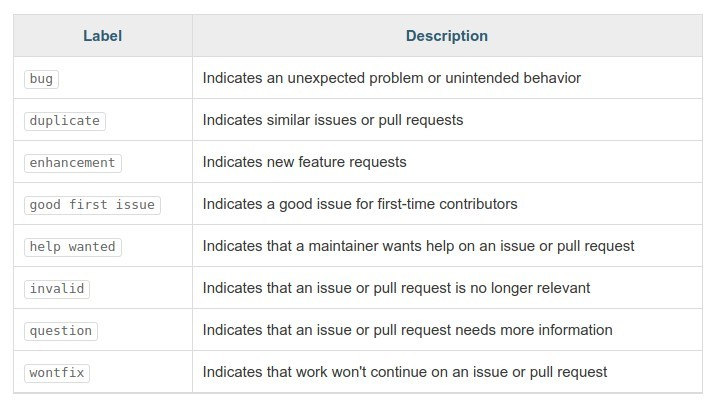
\includegraphics[width=8cm]{defaultLabels.jpg}
    \caption{Default Git labels provided for every repository}%
    \label{fig:defaultLabels}%
\end{figure}

From there I have chosen the label \textit{bug}. Then I have checked all custom tags of all repositories and chosen just those which were semantically similar to bug. All chosen labels can be seen in the table \ref{table:allGitBugLabels}


\begin{table}[H]
\centering
\begin{tabular}{ |p{3cm}||p{6cm}|}
 \hline
\textbf{ Repository }& \textbf{Chosen custom labels}\\
 \hline
 NodeJS   & confirmed-bug, errors \\ \hline
 AngularJS &   type: bug \\ \hline
 VueJS & browser-quirks, 1.x, 2.x\\ \hline
 Aurelia & enhancement\\ \hline
 EmberJS & Bug\\ \hline
\end{tabular}
\caption{Reddit submissions counts}
\label{table:allGitBugLabels}
\end{table}
